\section{Intelligent agents}
\label{sec:agents}

Unit~1 of the course studies two questions: who chooses an agent's next operation, and who decides
when the agent stops (\cref{sec:logistics}). These notes answer them for several agent
architectures, that is, several ways of organizing the decisions an agent makes. This section
supplies the vocabulary needed to compare them: what makes an agent rational, how we specify the
task an agent faces, and which property of that task makes it hard. We
apply each term to \msa{}, an agent that repairs one security weakness in code at a time and serves
as the course's running example.

\subsection{Rational agents}
\label{sec:agents-rational}

A rational agent is one that always chooses the action expected to do best by a standard of
success that we set for it. To state this precisely, we first define the terms the definition uses.

An \textbf{agent} is anything that perceives its \textbf{environment}, the part of the world around
it, and acts on that environment. What the agent senses at one moment is a \textbf{percept}. For a
software agent, a percept may be the text it receives after asking to read a file. The agent's
\textbf{percept sequence} is the complete history of everything it has perceived so far.

An \textbf{action} is something the agent does that can change its environment or what it perceives
next, such as reading a file or editing it. The \textbf{performance measure} is the criterion of
success: the standard by which we judge whether what the agent did was good. With these terms,
rationality is defined as follows.

\begin{definition}[Rational agent]
\label{def:agents-rational}
``For each possible percept sequence, a rational agent should select an action that is expected to
maximize its performance measure, given the evidence provided by the percept sequence and whatever
built-in knowledge the agent has.'' \citep[\S2.2.2]{russell2020aima}
\end{definition}

The definition asks for the action that is \emph{expected} to do best. It does not ask for the
action that turns out best. The expectation is formed from the evidence the agent has. An agent
that chooses well on its evidence is therefore rational even when the outcome depends on something
it could not perceive.

What is rational at any given time depends on four things:
\bi
\item \textbf{The performance measure.} It defines the criterion of success. Rationality depends on
it because an action can be the best one only by some standard. Under a different measure, a
different action can be the best one.
\item \textbf{Prior knowledge.} This is the built-in knowledge of the definition: what the agent
knows about its environment before it starts, for example how the code base is laid out.
Rationality depends on it because the agent forms its expectation of each action's result from this
knowledge together with its percepts.
\item \textbf{The available actions.} These are the actions the agent can perform. Rationality
depends on them because the agent can choose only among them, so the rational action is the best
action in this set.
\item \textbf{The percept sequence to date.} This is everything the agent has perceived up to the
moment of choice, and it grows with every new percept. Rationality depends on it because it is the
agent's evidence. The same agent can rationally choose differently after it has seen more.
\ei

The performance measure, the prior knowledge and the set of actions are all fixed before a run
begins. We write down the measure and the set of actions ourselves, and the prior knowledge
describes the world in which we place the agent. The percept sequence is the only factor that
changes while the agent runs.

We also keep the measure, the prior knowledge and the actions the same across these notes. The
architectures they compare therefore differ in one respect: how the agent's next action
depends on its percept sequence. The same difference can be stated in terms of time. The
architectures differ in which decisions we make at design time, before any run starts, and which
are made at run time, after the agent has seen its percepts.

In a fixed workflow, every step and every branch is written before the run. What the agent
perceives can change the next step only through a condition that we wrote in advance
(\cref{sec:fixed}). In a reactive loop, the agent chooses each next action after seeing the latest
percept (\cref{sec:reactive}).

\subsection{The running example: \msa{}}
\label{sec:agents-msa}

The course's running example is an agent called \msa{}, which repairs one reported security
weakness at a time. Its input comes from a \textbf{static-analysis scanner}, a program that reads
source code without running it and reports lines that match patterns of known weaknesses. Each
report is an \textbf{alert}: it names a file, a line and the kind of weakness suspected there.

\msa{} works on OWASP Benchmark\-Python, a Python web application made up of many small test cases.
Each test case is a short program that handles one kind of web request, and some test cases contain
deliberate security weaknesses.

The agent reads one alert as an \textbf{issue report}, a description of a problem that a developer
is asked to fix. It finds the flagged code, edits it, and submits a \textbf{patch}, the set of
changes it has made to the source files. A \textbf{run} is one execution of the agent on one alert.
In this design, a run ends when a submission passes a fixed set of checks, described below.

The agent acts through tools. A \textbf{tool} is an operation that the agent requests by name, with
arguments, and that another program carries out on its behalf. That program is the
\textbf{runtime}, the code that runs the agent: it executes each tool request, checks each
submission, and passes the results back to the agent.

\Cref{fig:agents-state} draws the whole agent as a \textbf{state machine}, a set of states with
transitions between them. Each state is one mode the agent can be in. Each transition is labeled
with the event that causes it, and the text in brackets names the information it carries. The
machine has three states and five transitions.
\bi
\item \textbf{Controller.} The Controller decides the next action. It either requests a tool,
passing the tool's name and arguments (\emph{tool requested}), or asks to submit, passing the
patch (\emph{submission requested}).
\item \textbf{Tool.} The Tool state runs the requested tool and returns its result to the
Controller (\emph{tool finished}). The result a tool returns is called an \textbf{observation}. An
observation is one kind of percept. The agent has three tools, drawn in \cref{fig:agents-state} as
a stack of boxes. The tool \demoref{read\_file} reads a range of lines from a file. The tool
\demoref{search} finds the places in the code that match a pattern. The tool \demoref{edit}
replaces one piece of text in a file with another.
\item \textbf{Submit.} The Submit state validates the submission with a fixed set of checks. If
the submission is \emph{accepted}, the run ends. If it is \emph{rejected}, the Submit state returns
feedback on the rejection to the Controller, which can continue working.
\ei

\begin{figure*}[t]
  \centering
  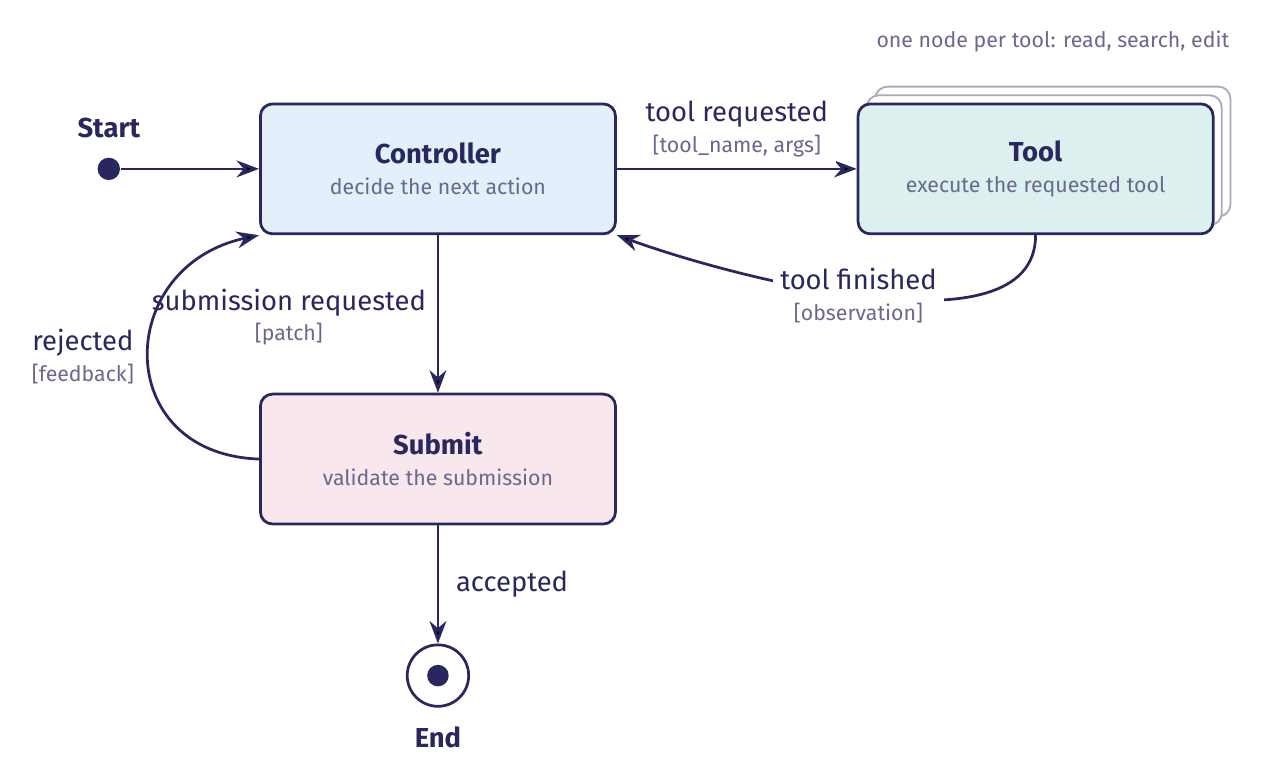
\includegraphics[width=0.8\textwidth]{figures/deck/state-graph.png}
  \caption{\msa{} as a state machine with three states (Controller, Tool and Submit) and five
  transitions. Each transition is labeled with the event that causes it, followed in brackets by
  the information it carries.}
  \label{fig:agents-state}
\end{figure*}

The Controller's decision can be made by code that we wrote or by a call to the model, the large
language model that generates text in reply to the text it is given (\cref{sec:logistics}). The
agent can ask the model to choose the next action.

Which of the two makes the Controller's decision depends on the architecture. Every architecture in
the rest of these notes is a variation on this machine: it adds or removes a state or a transition, or
changes which component makes a decision.

Later sections draw the machine as a graph, in which each state is a \textbf{node} and each
transition is an \textbf{edge}.

\subsection{A worked example: one SQL injection alert}
\label{sec:agents-run}

The alert we follow in these notes reports a possible SQL injection. In a \textbf{SQL injection}, a
value supplied by a user is inserted into the text of a database query, so that a crafted value can
change what the query does. The alert comes from Bandit, a static-analysis scanner for Python. It
flags a line that builds a query by \textbf{interpolation}, that is, by inserting a value directly
into the query string (\cref{lst:agents-before}).

\begin{lstlisting}[basicstyle=\ttfamily\footnotesize,caption={Before the fix: the value of \texttt{bar} is inserted into the query text.},label=lst:agents-before]
46  sql = f'SELECT username from USERS where password = \'{bar}\''
49  cur.execute(sql)
\end{lstlisting}

The listing omits lines~47 and~48, which open a connection to the database and create
\demoref{cur}, the cursor object through which line~49 sends the query. The variable
\demoref{bar} holds a value taken from the incoming request, so the user controls it.

Line~46 copies the characters of \demoref{bar} into the query text, and line~49 sends that text to
the database, which parses all of it as SQL. A quotation mark inside \demoref{bar} is therefore
read as part of the query's syntax. If a user sends the value
\lstinline[basicstyle=\ttfamily]{' OR '1'='1}, the condition becomes
\lstinline[basicstyle=\ttfamily]{password = '' OR '1'='1'}, which is true for every row, and the
query returns every username in the table.

The patch changes two lines (\cref{lst:agents-after}). Line~46 now holds a \textbf{placeholder},
the question mark, where the value used to be. Line~49 passes \demoref{bar} to the database as a
separate argument, called a \textbf{bound parameter}, rather than as part of the query text.

\begin{lstlisting}[basicstyle=\ttfamily\footnotesize,caption={After the fix: the query text holds a placeholder, and the value is passed separately as a bound parameter.},label=lst:agents-after]
46  sql = 'SELECT username from USERS where password = ?'
49  cur.execute(sql, (bar,))
\end{lstlisting}

The fix works because the database now receives the query text and the value separately. It first
parses the text, which contains no user input. Parsing settles the structure of the query before
any value is attached: which table is read, which column is compared and what condition selects the
rows. Only then does the database attach the value to the placeholder, as data to compare against
the password column. The characters of the value, quotation marks included, are never parsed as
SQL, so the value can no longer change the structure of the query.

\Cref{fig:agents-run} shows an example run of \msa{} on this alert, read from top to bottom. The
arrows that point to the Controller are percepts, and the arrows that point away from it are
actions. The first percept is the alert. The agent then reads the region around the flagged line,
and the result shows that line~46 interpolates \demoref{bar} and that line~49 executes the query.
The agent edits those two lines and submits a patch of two lines in one file.

At any point in the run, the agent's percept sequence consists of the arrows toward the Controller
above that point. It holds first the alert alone, then the alert and the excerpt that the read
returned, and so on. The edit also returns a confirmation, which is a percept, but the figure does not draw it.

\begin{figure*}[t]
  \centering
  \definecolor{navy}{HTML}{28285E}
  \definecolor{dblue}{HTML}{348EDC}
  \definecolor{dred}{HTML}{C73561}
  \begin{adjustbox}{width=0.9\textwidth}
  \begin{tikzpicture}[x=1cm, y=1cm, font=\sffamily\small, text=navy,
    head/.style={rounded corners=3pt, draw=navy, line width=0.8pt, fill=white,
                 minimum width=3.3cm, minimum height=0.8cm, font=\sffamily\small},
    life/.style={draw=black!45, dashed},
    act/.style={-{Stealth[length=2.8mm]}, line width=1.7pt, draw=dblue},
    per/.style={-{Stealth[length=2.8mm]}, line width=1.7pt, draw=dred},
    msg/.style={font=\sffamily\small, fill=white, inner sep=1.6pt, align=center, text=navy}]
    \node[head] (a) at (0,0) {Controller};
    \node[head] (r) at (15.4,0) {Runtime and tools};
    \draw[life] (a.south) -- (0,-5.5);
    \draw[life] (r.south) -- (15.4,-5.5);
    \draw[per] (15.4,-0.85) -- (0,-0.85) node[msg, midway, above] {alert: SQL injection at line 46};
    \draw[act] (0,-1.75) -- (15.4,-1.75) node[msg, midway, above] {\texttt{read\_file}: lines 40 to 52};
    \draw[per] (15.4,-2.65) -- (0,-2.65) node[msg, midway, above] {line 46 interpolates \texttt{bar}; line 49 executes the query};
    \draw[act] (0,-3.55) -- (15.4,-3.55) node[msg, midway, above] {\texttt{edit}: placeholder on line 46, \texttt{bar} bound on line 49};
    \draw[act] (0,-4.45) -- (15.4,-4.45) node[msg, midway, above] {\texttt{submit}: two lines, one file};
    \draw[per] (15.4,-5.3) -- (0,-5.3) node[msg, midway, above] {accepted: the patch passes every check. The run ends};
  \end{tikzpicture}
  \end{adjustbox}
  \caption{An example run of \msa{} on the worked alert, as messages between the Controller and the
  runtime. Arrows toward the Controller carry percepts, and arrows away from it carry actions.}
  \label{fig:agents-run}
\end{figure*}

The Submit state accepts the patch because the patch passes each of its checks, and the run then
ends.
\bi
\item \textbf{The patch applies.} Its changes can be made to the current files without conflict.
\item \textbf{The patch changes the flagged line.} Here, the flagged line is line~46.
\item \textbf{The rescan no longer reports the alert.} A \textbf{rescan} is a second run of the
scanner on the patched code. A rescan that no longer reports the alert is called \textbf{clean}.
\ei

\subsection{Why this is a rational agent}
\label{sec:agents-why-rational}

On the worked alert, \msa{} acts rationally when it reads the flagged code before editing it. To
check this claim, we first state, for our agent, the four things on which rationality depends.
\bi
\item \textbf{The performance measure.} The agent earns one point if its patch removes the
reported weakness and leaves the endpoint behaving as it did. The run must also stay within a limit
on its cost. An \textbf{endpoint} is a part of the application that answers one kind of request.
Here, it is the endpoint that contains the flagged code.
\item \textbf{Prior knowledge.} The agent knows the application's layout and what each tool
returns.
\item \textbf{The available actions.} The agent can call \demoref{read\_file}, \demoref{search} and
\demoref{edit}, and it can \demoref{submit} a patch.
\item \textbf{The percept sequence to date.} It is made up of the alert, whatever the tools return,
and the result of each submission. The agent perceives nothing else.
\ei

Given these four, the rational first action is to read the flagged lines before editing them. When
the agent makes its first choice, its percept sequence holds only the alert. The alert names a
file, a line and a kind of weakness, but it does not show the code. An \demoref{edit} names the
exact text it replaces, so an edit written without seeing the code could fail to apply, change the
wrong text, or alter what the endpoint returns.

A read costs one action and returns the code that the patch must change, including the exact text
that an edit has to name. Reading first is therefore the action expected to maximize the
performance measure. The read does not guarantee a correct patch. It makes one more likely, and the
definition judges the agent by its expected performance rather than by the outcome.

After the read, the percept sequence also holds the excerpt, and the rational choice changes. The
agent now knows which line builds the query and which line executes it, so editing those lines
becomes the action expected to do best. The same program chooses differently because its percept
sequence has grown.

The judgment that \msa{} is rational holds only relative to the four things listed above. If the
measure, the prior knowledge, the actions or the percepts change, a different action may become
the rational one. Rationality is therefore a property of a program together with these four, and
not of the program alone.

Stating the four also makes the claim that an agent is rational checkable. We can ask whether any
other available action was expected to do better under the same measure, knowledge and evidence.

\subsection{When the agent stops being rational}
\label{sec:agents-not-rational}

Behavior that is rational under one performance measure, or in one environment, can stop being
rational when either changes. Some behavior is not rational under our measure at all. In each of
the following cases, the behavior described does not maximize expected performance, and a better
agent behaves differently.
\bi
\item \textbf{Optimizing per tool call.} Suppose the measure also charges for each tool call, and a
call costs more the more text it returns. An agent that reads whole files then fares poorly,
because it pays for text it does not need. A better agent reads the smallest range of lines that
answers its question.
\item \textbf{Patching only the flagged line.} The weakness is the path by which an untrusted value
reaches the query. The flagged line is only the place where the scanner recognized one part of
that path. The value may reach the query through a helper function that the alert never names. A
patch to the flagged line alone can then leave part of that path in place, and the weakness
survives. A better agent first follows the value back to where it comes from.
\item \textbf{Editing after acceptance.} In \cref{fig:agents-state} the run ends at acceptance, so
this case arises only in a design that leaves the decision to stop to the agent. An agent that
keeps editing after its submission has been accepted gains nothing under the measure, and every
further edit risks breaking the endpoint's behavior. A better agent stops.
\ei

Each case becomes an explicit design decision in the architectures that follow:
\bi
\item \textbf{Cost.} In the reactive loop, the runtime enforces a \textbf{budget}, a limit on the
number of model calls a run may make. Once the budget is spent, the runtime refuses to issue
another model call (\cref{sec:reactive-stops}). Better tools also let the agent request only the
text it needs. Lecture~4 studies tools and their contracts.
\item \textbf{Depth of investigation.} In the planner, the plan sets how deep the investigation
goes (\cref{sec:planning}).
\item \textbf{Termination.} The decision to end a run becomes a stopping rule that we write and the
runtime applies, such as the budget and the stall check of the reactive loop
(\cref{sec:reactive-stops}). Lecture~3 returns to these rules and asks when they guarantee that a
run ends.
\ei

A separate gap lies in the checks rather than in the agent. The Submit state checks less than the
performance measure asks. It checks that the patch applies, that it changes the flagged line, and
that the rescan no longer reports the alert. The measure asks that the weakness be gone and that
the endpoint still behave as it did.

No check runs the endpoint. A rescan that reports nothing shows only that the scanner no longer
recognizes the pattern it flagged. An accepted submission is therefore not necessarily a correct
one. A patch to the flagged line alone, when the unsafe value comes from a helper function, can pass
every check while the weakness survives.

\subsection{The task environment}
\label{sec:agents-environment}

Before designing an agent, we write down the task it must perform. That specification is the
\textbf{task environment}. It has four parts, a performance measure (P), an environment (E),
actuators (A) and sensors (S), and is written down as a \textbf{PEAS description}
\citep[\S2.3.1]{russell2020aima}.
\bi
\item \textbf{Performance measure.} It states what counts as success.
\item \textbf{Environment.} It is the world in which the agent acts.
\item \textbf{Actuators.} They are the means by which the agent acts on its environment. For a
software agent, they are the operations it can request, such as its tools. An action is one use of
an actuator, for example one call to \demoref{read\_file} with a particular path and range.
\item \textbf{Sensors.} They are the means by which the agent perceives its environment. For a
software agent, they are the channels through which inputs and results are handed back to it. A
percept is what arrives through a sensor at one moment, for example the lines that one read
returned.
\ei

In our task environment, the code base is taken at a \textbf{pinned commit}, one fixed version of
its history, so that every run starts from the same files. The \textbf{working tree} is the copy of
those files that the agent reads and edits during a run. Among the sensors, the \textbf{validation
result} is the Submit state's verdict on a submission: accepted, or rejected with feedback.

\Cref{tab:agents-peas} fills in the four parts for \msa{}. In the table, the performance measure
asks for a correct patch at bounded cost, that is, within a limit on what the run may spend. The
actuators are exactly the agent's tools and its submission.

\begin{table}[htbp]
  \caption{PEAS description of the task environment for \msa{}.}
  \label{tab:agents-peas}
  \begin{adjustbox}{width=\linewidth}\begin{tabularx}{\linewidth}{L{0.27\linewidth}X}
    \toprule
    & \textbf{For \msa{}} \\
    \midrule
    \textbf{Performance measure} & The reported weakness is gone, and the endpoint still returns
    what it returned before, at bounded cost \\
    \textbf{Environment} & OWASP BenchmarkPython at a pinned commit, one scanner alert read as an
    issue report, and the working tree the agent edits \\
    \textbf{Actuators} & \demoref{read\_file(path,~range)}, \demoref{search(pattern)},
    \demoref{edit(path,~old,~new)}, \demoref{submit(patch)} \\
    \textbf{Sensors} & The alert, file excerpts, search hits, edit confirmations, the validation
    result, and tool errors \\
    \bottomrule
  \end{tabularx}\end{adjustbox}
\end{table}

We specify the task environment as fully as possible before designing the agent, because the right
design depends on it. A property of the task, such as how much of it the agent can see, determines
what the agent must do, for example whether it must act to gather information
(\cref{sec:agents-properties}). The architectures in the rest of these notes all keep the task
environment of \cref{tab:agents-peas} fixed and differ only in how the agent chooses its actions.

\subsection{Properties of the task environment}
\label{sec:agents-properties}

A task environment can be classified along seven dimensions, each a pair of opposite properties
\citep[\S2.3.2]{russell2020aima}. Where a task sits on each dimension tells us what the agent must
cope with. Each table below gives the definitions of the two properties and places familiar tasks
on each side. The tasks include solving a crossword, playing chess or poker, driving a taxi and
diagnosing a patient.

Several of the definitions refer to the state of the environment. The \textbf{state} of an
environment is everything about it at one moment that can matter to the task, for example the
current contents of every file. This is a different use of the word from the states of
\cref{fig:agents-state}, which are modes of the agent.

On each dimension, one side makes an agent easier to design: fully observable, single agent,
deterministic, episodic, static, discrete and known. Our task environment is on the easier side of
every dimension except observability and the episodic or sequential dimension. It is partially
observable, and it is sequential within one alert but episodic across alerts. Partial observability
is the property that makes the task hard, as the first dimension below explains.

% Each property is a heading, an explanation, an uncaptioned table (so that the PEAS and vocabulary
% tables stay Tables 1 and 2, as slide 34 says) and the verdict. \nopagebreak keeps the heading with
% its explanation; the fil pair before each heading lets a column end short there instead of
% stretching its glue.
\par\vskip 0pt plus 1fil\penalty500\vskip 0pt plus -1fil\relax
\paragraph{Fully or partially observable.}\leavevmode\par\nopagebreak
This dimension asks whether the agent's sensors show it everything it needs in order to choose an
action. An environment is \textbf{fully observable} when they do, and \textbf{partially observable}
when some relevant part of the state is hidden or reported inaccurately. A crossword is fully
observable, because the whole grid is in front of the solver. Poker is partially observable,
because the other players' cards are hidden.
\par\nopagebreak\smallskip
\noindent\begin{adjustbox}{width=\linewidth}\begin{tabularx}{\linewidth}{L{0.2\linewidth}XX}
  \toprule
  & \textbf{Fully observable} & \textbf{Partially observable} \\
  \midrule
  \textbf{Definition} & The sensors give the agent the complete state of the environment at each
  point in time, or at least every part that matters for the choice of action. & The sensors are
  noisy or inaccurate, or part of the state is simply missing. With no sensors at all, the
  environment is unobservable. \\
  \textbf{Examples} & Crossword, chess with a clock, backgammon, image analysis & Poker, taxi
  driving, medical diagnosis, part-picking robot, refinery controller \\
  \bottomrule
\end{tabularx}\end{adjustbox}\par
Our task environment is partially observable. The agent sees only the parts of the code that it
reads. It never sees whether the endpoint still works, because none of its actions runs the
application. Nor does it see the setting in which the application is deployed: the machine that
runs it, the operating system, or the other programs running beside it.

This property is what makes the task hard. The evidence a correct patch depends on, such as where
an unsafe value comes from, reaches the agent only through actions it chooses to take. In a
partially observable environment, a rational agent must therefore act in order to gather
information, as \msa{} does when it reads before it edits.

\par\vskip 0pt plus 1fil\penalty500\vskip 0pt plus -1fil\relax
\paragraph{Single agent or multiagent.}\leavevmode\par\nopagebreak
This dimension asks whether any other entity in the environment is pursuing a goal that depends on
what our agent does. The environment is \textbf{single agent} when no such entity exists, and
\textbf{multiagent} when one does. A crossword is single agent. Chess is multiagent and
competitive, because the opponent's success depends on our moves. Traffic is multiagent and partly
cooperative, because drivers try to avoid colliding with one another.
\par\nopagebreak\smallskip
\noindent\begin{adjustbox}{width=\linewidth}\begin{tabularx}{\linewidth}{L{0.2\linewidth}XX}
  \toprule
  & \textbf{Single agent} & \textbf{Multiagent} \\
  \midrule
  \textbf{Definition} & No other entity behaves as though it were maximizing a measure that
  depends on what this agent does. & Another entity is best described as maximizing a measure whose
  value depends on this agent's behavior. It can compete, as in chess, or cooperate, as in
  traffic. \\
  \textbf{Examples} & Crossword, medical diagnosis, image analysis, part-picking robot, refinery
  controller & Chess with a clock, poker, backgammon, taxi driving, English tutor \\
  \bottomrule
\end{tabularx}\end{adjustbox}\par
Our task environment is single agent. The working tree, the tools and the Submit checks respond to
the agent's actions, but none of them pursues a goal of its own. Nothing the agent interacts with
is trying to cooperate with it or to beat it.

\par\vskip 0pt plus 1fil\penalty500\vskip 0pt plus -1fil\relax
\paragraph{Deterministic or nondeterministic.}\leavevmode\par\nopagebreak
This dimension asks whether the current state and the agent's action together settle the result of
the action. In a \textbf{deterministic} environment, the current state and the agent's action
completely determine the next state. In a \textbf{nondeterministic} environment they do not, so the
same action in the same state can lead to different results. Filling in a square of a crossword has
exactly one result. A move in backgammon depends on a roll of the dice.

By convention, uncertainty that comes only from another agent's choices does not count, which is
why chess appears in the deterministic column. A \textbf{stochastic} environment is a
nondeterministic one in which the possible results are given probabilities. A partially observable
environment can look nondeterministic even when it is not, because the part of the state that
decides the result is hidden from the agent.
\par\nopagebreak\smallskip
\noindent\begin{adjustbox}{width=\linewidth}\begin{tabularx}{\linewidth}{L{0.2\linewidth}XX}
  \toprule
  & \textbf{Deterministic} & \textbf{Nondeterministic} \\
  \midrule
  \textbf{Definition} & The current state and the action the agent executes fix the next state
  completely. & They do not. A partially observable environment can look nondeterministic even when
  it is not. Stochastic is the narrower word, for models that put numbers on the possibilities. \\
  \textbf{Examples} & Crossword, chess with a clock, image analysis & Poker, backgammon, taxi
  driving, medical diagnosis, refinery controller \\
  \bottomrule
\end{tabularx}\end{adjustbox}\par
Our task environment is deterministic: the same read, or the same rescan, on the same files returns
the same result every time. Determinism is a property of the environment, and it does not mean that
every run of the agent takes the same path. The model's replies are \emph{sampled}: the model draws
each reply at random from a range of likely replies, so the same request can produce different
replies. An edit also changes the files that later reads return. Two runs from the same state can
therefore still take different paths, as the example run of the reactive loop shows
(\cref{sec:reactive-run}).

\par\vskip 0pt plus 1fil\penalty500\vskip 0pt plus -1fil\relax
\paragraph{Episodic or sequential.}\leavevmode\par\nopagebreak
This dimension asks whether the agent's current decision affects its later ones. In an
\textbf{episodic} environment, experience divides into separate episodes. In each one the agent
perceives and then acts once, and no episode depends on the actions taken in earlier ones. In a
\textbf{sequential} environment, the current decision can affect every decision that follows. A
part-picking robot that sorts parts from a conveyor belt works episodically, because each part is
judged on its own. Chess is sequential, because each move constrains the moves that follow.
\par\nopagebreak\smallskip
\noindent\begin{adjustbox}{width=\linewidth}\begin{tabularx}{\linewidth}{L{0.2\linewidth}XX}
  \toprule
  & \textbf{Episodic} & \textbf{Sequential} \\
  \midrule
  \textbf{Definition} & Experience divides into separate episodes. The agent perceives, then acts
  once, and the next episode owes nothing to the last. & The current decision can affect every
  decision that follows. \\
  \textbf{Examples} & Image analysis, part-picking robot & Crossword, chess, poker, backgammon, taxi
  driving, medical diagnosis, refinery controller, English tutor \\
  \bottomrule
\end{tabularx}\end{adjustbox}\par
Our task environment is both, at different scales. It is sequential within one alert, because what
the agent reads next depends on what it has just read, and an edit changes what later reads return.
It is episodic across alerts if we treat the whole run on one alert as a single episode. No run
depends on an earlier one, because the agent carries nothing from one alert to the next.

\par\vskip 0pt plus 1fil\penalty500\vskip 0pt plus -1fil\relax
\paragraph{Static or dynamic.}\leavevmode\par\nopagebreak
This dimension asks whether the environment can change while the agent is deciding what to do. A
\textbf{static} environment cannot, so the time the agent spends deciding costs it nothing. A
\textbf{dynamic} environment can, as traffic does while a taxi driver hesitates. An environment is
\textbf{semidynamic} when the environment itself does not change with time but the agent's score
does, as in chess played with a clock.
\par\nopagebreak\smallskip
\noindent\begin{adjustbox}{width=\linewidth}\begin{tabularx}{\linewidth}{L{0.2\linewidth}XX}
  \toprule
  & \textbf{Static} & \textbf{Dynamic} \\
  \midrule
  \textbf{Definition} & The environment cannot change while the agent is thinking, so time spent
  deciding costs nothing. & The environment can change while the agent is thinking. Semidynamic if
  the environment does not change with time but the score does. \\
  \textbf{Examples} & Crossword, poker, backgammon; chess with a clock and image analysis are
  semidynamic & Taxi driving, medical diagnosis, part-picking robot, refinery controller, English
  tutor \\
  \bottomrule
\end{tabularx}\end{adjustbox}\par
Our task environment is static. The working tree changes only when the agent edits it, so nothing
changes while the agent is deciding what to do next.

\par\vskip 0pt plus 1fil\penalty500\vskip 0pt plus -1fil\relax
\paragraph{Discrete or continuous.}\leavevmode\par\nopagebreak
This dimension asks whether the state, time, percepts and actions take a finite number of distinct
values. In a \textbf{discrete} environment they do, as the positions and moves of chess do. In a
\textbf{continuous} environment they range smoothly over values, as the speed and position of a
taxi do.
\par\nopagebreak\smallskip
\noindent\begin{adjustbox}{width=\linewidth}\begin{tabularx}{\linewidth}{L{0.2\linewidth}XX}
  \toprule
  & \textbf{Discrete} & \textbf{Continuous} \\
  \midrule
  \textbf{Definition} & The state, the handling of time, and the agent's percepts and actions all
  come in a finite number of distinct values. & State, time, percepts or actions sweep through a
  range of values. \\
  \textbf{Examples} & Crossword, chess with a clock, poker, backgammon, English tutor & Taxi
  driving, medical diagnosis, image analysis, part-picking robot, refinery controller \\
  \bottomrule
\end{tabularx}\end{adjustbox}\par
Our task environment is discrete. Files, lines, edits and \textbf{hunks}, the blocks of changed
lines that make up a patch, can all be counted. Nothing in the task is a quantity measured on a
continuous scale.

\par\vskip 0pt plus 1fil\penalty500\vskip 0pt plus -1fil\relax
\paragraph{Known or unknown.}\leavevmode\par\nopagebreak
This dimension concerns what is known about how the environment works, rather than the environment
itself. An environment is \textbf{known} when the agent, or its designer, knows the rules that
govern it: what result each action produces in each state, or with what probabilities. It is
\textbf{unknown} when the agent must first learn those rules before it can choose well.

Knowing the rules does not mean knowing the current state. Whether the agent can see the current
state is the separate question of observability. A new video game shows the whole screen, so it is
fully observable. It does not say what the buttons do, so it is unknown.
\par\nopagebreak\smallskip
\noindent\begin{adjustbox}{width=\linewidth}\begin{tabularx}{\linewidth}{L{0.2\linewidth}XX}
  \toprule
  & \textbf{Known} & \textbf{Unknown} \\
  \midrule
  \textbf{Definition} & The outcomes of every action are given. This is about what the agent
  knows, not about the environment itself. & The agent has to learn how the world works before it
  can choose well. A new video game shows the whole screen and still will not say what the buttons
  do. \\
  \textbf{Examples} & Chess and poker: the rules can be handed over in full & Driving a rented car
  in a country you have not driven in \\
  \bottomrule
\end{tabularx}\end{adjustbox}\par
Our task environment is known, because we know what each tool does. What the agent does not know is
where the weakness is and how the unsafe value reaches it. That is a matter of observability rather
than of knowing how the world works: the information is in the code, but the agent sees it only by
reading.

\subsection{The agent, its tools, and its environment}
\label{sec:agents-picture}

\begin{figure*}[t]
  \centering
  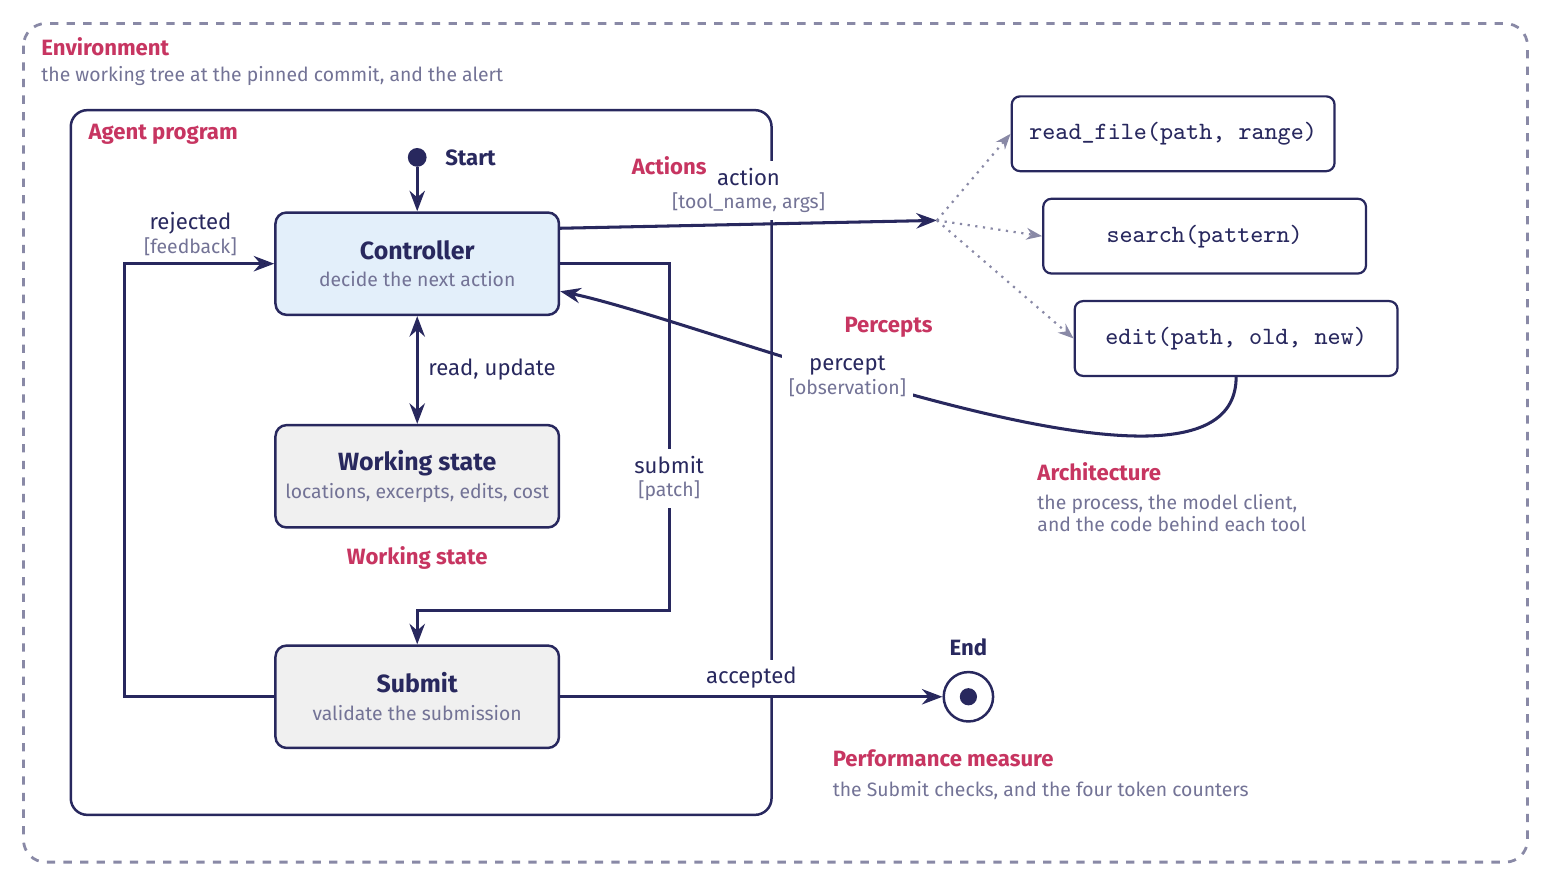
\includegraphics[width=\textwidth]{figures/deck/state-graph-annotated.png}
  \caption{\msa{} inside its environment: the state machine of \cref{fig:agents-state}, with the
  working state drawn and one box per tool. Each label in magenta names a row of
  \cref{tab:agents-vocabulary}.}
  \label{fig:agents-annotated}
\end{figure*}

The terms of \cref{tab:agents-vocabulary} each name a part of \msa{} or of its environment.
\Cref{fig:agents-annotated} shows these parts by placing the state machine of
\cref{fig:agents-state} inside its environment. Each label in magenta names a term that
\cref{tab:agents-vocabulary} defines for our agent. The figure adds the following to
\cref{fig:agents-state}.
\bi
\item \textbf{The environment.} The dashed outer box is the environment: the working tree at the
pinned commit, and the alert.
\item \textbf{The working state.} The Controller reads and updates a \textbf{working state}, the
agent's own record of what the run has found so far: code locations, excerpts, edits and cost.
\Cref{fig:agents-state} did not draw it.
\item \textbf{One box per tool.} The Tool state is split into one box per tool, reached by dotted
lines, because the Controller requests a tool by its name.
\ei

The solid box is the \textbf{agent program}, the code that chooses the agent's actions from its
percepts. It contains the Controller, the working state and the Submit state.

The agent program runs on machinery that executes it and carries out its actions. This machinery
consists of the operating-system process that runs the program, the \textbf{model client} (the code
that sends requests to the model), and the code behind each tool. In the vocabulary of
\cref{tab:agents-vocabulary}, this machinery is called the \textbf{architecture}. Everywhere else in
these notes, \emph{architecture} has a different meaning: a way of organizing the agent program,
such as a fixed workflow or a reactive loop.

The figure also shows how the agent program reaches its environment and how a run ends.
\bi
\item \textbf{Access to the environment.} Apart from the Submit checks, which run the scanner on
the working tree, the tools are the only way the agent program reaches the environment. Every
percept after the alert, other than the verdict on a submission, comes back from a tool, and every
change to the working tree is made by the \demoref{edit} tool.
\item \textbf{Ending a run.} The only transition to the end leaves the Submit state, so in this
machine a run ends only when a submission is accepted. Later architectures add other ways to stop
a run, such as a budget (\cref{sec:reactive-stops}).
\ei

The size of a model's input and output is measured in \textbf{tokens}, small pieces of text that
are often parts of words. Four counters record how many tokens the run has used, one for each kind
of token that the model's provider reports, such as input and output tokens. The counters track the
cost that the measure bounds. Lecture~3 shows how the runtime adds the tokens of each model call to
them.

The performance measure is not part of the agent program. It is our standard for judging a run
from outside the program. Inside the program, the Submit checks and the token counters stand in
for parts of it. The Submit checks test part of what the measure asks, though less than all of it
(\cref{sec:agents-not-rational}).

\Cref{tab:agents-vocabulary} lists each term with the part of \msa{} it names.

\begin{table}[htbp]
  \caption{The vocabulary of intelligent agents, with the part of \msa{} that each term names. Each
  row matches a label in magenta in \cref{fig:agents-annotated}.}
  \label{tab:agents-vocabulary}
  \begin{adjustbox}{width=\linewidth}\begin{tabularx}{\linewidth}{L{0.27\linewidth}X}
    \toprule
    \textbf{Term} & \textbf{In \msa{}} \\
    \midrule
    \textbf{Environment} & The working tree at the pinned commit, and the alert \\
    \textbf{Agent program} & The Controller, which decides the next action; the working state it
    reads and updates; and the Submit state, which validates the submission \\
    \textbf{Working state} & Locations, excerpts, edits, cost \\
    \textbf{Actions} & \demoref{read\_file(path,~range)}, \demoref{search(pattern)} and
    \demoref{edit(path,~old,~new)}, each requested by name with its arguments, and \demoref{submit}
    with a patch \\
    \textbf{Percepts} & The alert, file excerpts, search hits, edit confirmations, the validation
    result, and tool errors \\
    \textbf{Architecture} & The process, the model client, and the code behind each tool \\
    \textbf{Performance measure} & The Submit checks, and the four token counters \\
    \bottomrule
  \end{tabularx}\end{adjustbox}
\end{table}

\subsection{The architectures that follow}
\label{sec:agents-route}

The rest of these notes takes \msa{} through a sequence of architectures. The fixed workflow, the
reactive loop and the planner let the agent decide progressively more of its run for itself. The
validator then adds a separate model call that judges a patch only after the Submit checks have
passed it.
\bi
\item \textbf{Fixed workflow.} We write every step and its order before the run, and the model
only supplies content at the points we choose (\cref{sec:fixed}).
\item \textbf{Reactive loop (ReAct, short for reasoning and acting).} The model chooses the next
action after seeing each result. Its graph has the edge from the tools back to the Controller that
\cref{fig:agents-state} draws, and the fixed workflow's graph lacks it (\cref{sec:reactive}).
\item \textbf{Planner.} The agent writes its intended sequence of steps into its working state,
where the plan can be read and revised as the run proceeds (\cref{sec:planning}).
\item \textbf{Validator.} A new node, the validator, judges each patch that has passed the Submit
checks, and it becomes the one component that can end a run with an accepted patch
(\cref{sec:validation}).
\item \textbf{Other agent architectures.} The notes close with a survey of further architectures
from a catalogue of agentic design patterns (\cref{sec:patterns}).
\ei

Across these architectures, the agent's task, the alert and the tools stay the same, and only the
architecture changes. This is what makes the comparison worth making. A difference between two
architectures on the same alert cannot then be explained by a change in the task or the tools.

\subsection*{Key points}
\bi
\item A rational agent selects, for each percept sequence, the action expected to maximize its
performance measure, given the evidence of its percepts and its built-in knowledge.
\item Rationality depends on the performance measure, prior knowledge, the available actions and
the percept sequence to date, so it is a property of a program relative to these four rather than
of the program alone.
\item Reading the flagged code before editing it is the rational first action for \msa{}, because
the environment is partially observable and the code reaches the agent only through its own reads.
\item The Submit checks test less than the performance measure asks, so an accepted patch is not
necessarily a correct one.
\item A task environment is specified by its performance measure, environment, actuators and
sensors (PEAS), and specifying it fully comes first because the right design depends on it.
\item Our task environment is partially observable, single agent, deterministic, static, discrete
and known, and it is sequential within one alert and episodic across alerts.
\item The architectures in these notes keep the task environment fixed and differ only in how the
agent's next action depends on its percept sequence.
\ei
